\documentclass[12pt,a4paper]{article}
\usepackage[utf8]{inputenc}
\usepackage[vietnamese=nohyphenation]{hyphsubst}
\usepackage[vietnamese]{babel}
\usepackage[autostyle]{csquotes}
%\MakeOuterQuote{"}
\usepackage{graphicx}
\graphicspath{ {image/} }

%opening
\title{Blockchain}
\author{Nguyễn Lễ}

\begin{document}

\maketitle

\begin{abstract}

\end{abstract}

\section{Lịch sử blockchain}

Blockchain được công chúng biết tới lần đầu tiên khi Satoshi Nakamoto, người mà danh tính thật sự  vẫn chưa ai biết, đăng bài báo cáo Bitcoin: A Peer to Peer Electronic Cash System vào năm 2008, trong đó mô tả một 'phiên bản mạng ngang hàng của tiền mã hóa' được gọi là Bitcoin.  Blockchain, công nghệ mà Bitcoin chạy trên  , đã phát triển trong suốt thập niên qua, thành một trong những công nghệ đột phá lớn nhất với tiềm năng tác động đến mọi ngành từ tài chính đến sản xuất. Dưới đây là một lịch sử ngắn gọn về công nghệ blockchain:

\subsection{Khởi đầu với Bitcoin}
Ta không thể  nói về lịch sử của blockchain mà không bắt đầu bằng việc nói về Bitcoin. Sau khi báo cáo của Nakamoto được đăng, Bitcoin được cung cấp cho cộng đồng mã nguồn mở trong năm 2009. Blockchain cung cấp giải pháp cho vấn đề sự tin tưởng trong thế giới số bởi vì bất kỳ ai cũng có thể xem thông tin mà nó ghi lại và không cho phép bất kỳ ai xóa chúng. Nó có tinh minh bạch, có ghi lại thời gian và có tính phi tập trung.

%“Blockchain dùng cho Bitcoin, như internet dùng cho email. Một hệ thống điện tử lớn, mà bạn có thể xây ứng dụng trên đó. Tiền tệ chỉ là một trong số chúng” Sally Davies, FT Technology reporter.

\subsection{Blockchain tách ra từ Bitcoin}

Ngay cả ngày hôm nay, có rất nhiều người tin rằng Bitcoin và blockchain là một và như nhau, mặc dù không phải thế. Trong năm 2014, nhiều người bắt đầu nhận ra  rằng blockchain có thể được sử dụng không chỉ cho tiền mã hóa mà còn cho nhiều thứ khác, bắt đầu đầu tư và nghiên cứu làm thế nào để sử dụng blockchain để thay đổi  quy trình hoạt động trong các lĩnh vực khác nhau. Cốt lõi của blockchain là một sổ cái mở, phi tập trung, ghi lại các giao dịch giữa hai bên một cách liên tục mà không cần xác thực của bên thứ ba. Điều này giúp tăng tính hiệu quả và làm giảm đáng kể chi phí giao dịch.

Khi các doanh nhân hiểu được sức mạnh của blockchain, đã có một sự gia tăng đầu tư và nghiên cứu để xem làm thế nào để ứng dụng blockchain vào chuỗi cung ứng, y tế, bảo hiểm, vận chuyển, bầu cử, quản lý hợp đồng và nhiều hơn nữa. Gần 15\% các tổ chức tài chính hiện tại đang sử dụng công nghệ blockchain. 

\subsection{Sự nổi lên của Ethereum: Hợp đồng thông minh}

Vitalik Buterin, đồng sáng lập  Ethereum và tạp chí Bitocoin, cũng là một trong những người đóng góp cho hệ thống codebase Bitcoin những ngày đầu tiên, nhưng bắt đầu nản lòng trong  2013 bởi sự hạn chế về lập trình của nó và thúc đẩy cải tiến nó trở nên mềm dẻo hơn. Gặp phải sự phản đối từ cộng đồng Bitcoin, Buterin bắt đầu xây dựng một blockchain mở thứ hai gọi là Ethereum. Sự khác biệt lớn nhất giữa hai blockchain là Ethereum có thể ghi chép lại không chỉ tiền tệ mà còn các tài sản khác như là các khoản vay hoặc hợp đồng. Ethereum ra mắt vào năm 2015 và có thể được sử dụng để xây dựng “hơp đồng thông minh”—có thể tự động xử lý dựa trên một bộ quy tắc được thiết lập trong blockchain Ethereum. Công nghê này đã thu hút sự chú ý của các tập đoàn như Microsoft, BBVA và UBS, bị lôi cuốn bởi tiềm năng giúp tiết kiệm thời gian và tiền bạc của hợp đồng thông minh.

\subsection{Sự chuyển dịch sang Proof of Stake}

Hiện tại, công nghệ blockchain hoạt động dựa trên cơ chế ''chứng minh theo công sức'' (proof of work, POW): để tạo một block cần phải dùng đến khả năng tính toán của một máy tính đắc tiền. Các giao địch sẽ được đóng gói lại thành một block. Sau đó các máy đào (miner) sẽ xác nhận các giao dịch trong block có đúng với các quy tắc đề ra hay không bằng cách giải một bài toán POW, một bài toán rất khó đòi hỏi một khối lượng sức mạnh tính toán đặc biệt để giải. Máy đào đầu tiên giải được bài toán đó sẽ nhận được phần thưởng và sau đó các giao dịch được chứng thực sẽ được lưu trữ trong blockchain. Các nhà phát triển Ethereum quan tâm đến việc chuyển sang một cơ chế đồng thuận mới gọi là ''chứng minh theo cổ phần'' (proof of stake, POS).

POS có  cùng mục tiêu với POW: xác nhận các giao dịch và đạt được sự đồng thuận trong chuỗi thông quan việc sử dụng một thuận toán khác.  Với POS, người tạo ra block mới ''được chọn theo một cách xác định, tùy thuộc vào lượng tài sản (trong blockchain) mà người nó nắm giữ, hay trong POS được gọi là cổ phần (stake).''  Những người ủng hộ sự thay đổi này, bao gồm đồng sáng lập Ethereum, Buterin, thích cơ chế POS do cơ chế này giúp tiết kiệm năng lượng và chi phí hơn so với POW.

\subsection{Nhân rộng Blockchain}
Do hiện tại, mọi máy tính trong một blockchain đều phải xử lý mọi giao dịch, nên quá trình này có thể diễn ra rất chậm. Một giải pháp nhân rộng Blockchain sẽ xác định xem cần bao nhiêu máy tính để xác thực một giao dịch mà không ảnh hưởng đến vấn đề bảo mật.

Ngày nay, Bitcoin chỉ là một trong hàng trăm ứng dụng sử dụng công nghệ blockchan. Sự thay đổi của công nghệ blockchain đã trải qua một thập kỷ và ta không thể nào tiên đoán được thập kỷ kế tiếp blockchain sẽ thay đổi đến mức nào.

\section{Khái niệm về blockchain}
\subsection{Công nghệ sổ cái phân tán (Distrubed Ledger Technology) và Blockchain}

%Một sổ cái phân tán là một cơ sở dữ liệu truyền qua nhiều nút hoặc thiết bị vi tính. Mỗi nút sao chép và lưu lại một bản sao của sổ cái. Mỗi node tham gia mạng đều cập nhật một sổ cái độc lập.
%
%Tính năng đột phá của công nghệ sổ cái phân tán là sổ cái này không được duy trì bởi bất kỳ cơ quan trung tâm nào. Việc cập nhật sổ cái được thiết lập và ghi lại một cách độc lập bởi mỗi nút. Các nút sau đó bỏ phiếu chọn ra một phiên bản cập nhất chung để đảm bảo rằng đa số đồng ý với kết luận đạt được.   Việc bỏ phiếu và thoản thuận chọn ra một bản sao chép của số cái được gọi là sự đồng thuận., và được tiến hành bởi một thuận toán đồng thuận. Một khi đã đạt được sự đồng thuận, sổ cái phân tán sẽ cập nhật chính nó và phiên bản mới nhất, được đồng thuận  sẽ được lưu vào mỗi nút riêng biệt.
%
%Công nghệ sổ cái phân tán giảm đáng kể chi phí tin tưởng. Kiến trúc và cấu trúc của sổ cái phân tán có thể giúp chúng ta giảm bớt sự phụ thuộc vào ngân hàng, chính phủ, luật sư, công chứng viên và viên chức nhà nước. Corda của R3 là một ví dụ của một sổ cái phân tán.
%
%Các sổ cái phân tán thể hiện một mô hình mới về cách thức thu thập và truyền đạt thông tin, và sẵn sàng cho cuộc cách mạng hóa cách thức các cá nhân, doanh nghiệp và chính phủ giao dịch.

Công nghệ Sổ cái phân tán (DLT) nhận được ngày càng nhiều sự chú ý trong những năm gần đây như một phương pháp mới giúp lưu trữ và cập nhật dữ lữu trong và giữa các tổ chức. Một sổ cái phân tán là một sổ cái số, khác biệt so với mạng tập trung và hệ thống sổ truyền thống ở hai điểm: Đầu tiên, thông tin được lưu trữ trong một mạng lưới các máy tính mà ở đó các thay đổi xảy ra với một sổ cái trong mạng sẽ được phản ánh đồng thời đến tất cả chủ sỡ hữu sổ cái khác. Thứ hai, thông tin được  xác nhận bởi một chữ ký điện tử. Những hệ thống này cùng nhau cung cấp một bản ghi giao dịch minh bạch và có thể kiểm tra lại. 

Công nghệ blockchain là một trong những ứng dụng được biết đến nhiều nhất của DLT, trong đó sổ cái bao gồm các khối (block) chứa các giao dịch, nó là công nghệ nền tảng của Bitcoin. Tuy nhiên, các ứng dụng khả dĩ của DLT đã lan tới lĩnh vưc giáo dục, các ngàng công nghệ sáng tạo, và các ngành nông nghiệp và thực phẩm.

Những tính năng chính của Blockchain,  thứ làm nó khác biệt so với các loại cơ sở dữ liệu khác, xuất phát từ bản chất ''phân tán'' của nó. Trong blockchain, mỗi nút trong blockchan đều giữ một phiên bản sổ của riêng họ, dữ liệu được thêm vào nhờ thuật toán đồng thuận và không cần bên thứ ba. Kết quả là, Blockchain có thể cung cấp nhiều lợi ích trong các vấn đề về tính hiệu quả, niềm tin và đối chiếu dữ liệu giữa tất cả sổ cái trong blockchain. Điều này có nghĩa là Blockchin có thể cung cấp:
\begin{itemize}
	\item \textit{Một bản ghi không thể thay đổi được:} Dữ liệu được thêm vào sổ cái không thể thay đổi, được bảo vệ và hiện diện trong suốt vòng đời của sổ cái, nếu như được đồng thuận bởi mọi thành viên
	 \item \textit{Khả năng phi trung gian:} Các nút có khả năng tương tác trực tiếp mà không cần đến một bên trung gian. Điều này bao gồm khả năng khởi tạo các giao dịch dữ liệu hoặc tài sản đã được số hóa (có thể là một loại tiền tệ, chẳng hạn như bitcoin, hoặc một đại diện số của tài sản thực, ví dụ như quyền sở hữu đất hoặc tiền thật).
	\item \textit{Không bị điều khiển bởi một cá thể trung tâm:} Việc thêm dữ liệu vào sổ cái hoặc thay đổi cấu trúc điều hành phải được quyết định dựa sự đồng thuận của các bên tham gia.
	\item \textit{Cơ hội mói cho việc quản lý và chia sẽ dữ liệu.} Việc truy cập dữ liệu giữa các bên tham gia dễ dàng hơn sẽ tạo ra nhiều ứng dụng cho việc quản lý và chia sẽ dữ liệu. 
\end{itemize}

\subsection{Các loại Blockchain}
%Sổ Không Cần Cho Phép (Permisionless) hay Sổ Công Cộng (Public) được xem như một torng những dạng ''nguyên thủy nhất'' của Blockchain.  Một ví dụ điển hình chính là Blockchain, công nghệ nền tảng của Bitcoin. Trong loại cấu hình này, những người tham gia ''không cần được cho phép'' và bất kỳ ai cũng có thể tham gia và thực hiện xác thực giao dịch với đầy đủ quyền. Những người tham gia được xác định thông qua tên giả hoặc được gữ kín, 
Một blockchain có thể là permisionless (không cần cho phép) (như Bitcoin hoặc Ethereum) hoặc permissioned (cần cho phép)). Một blockchain không cần cho phép, còn được gọi là một blockchain công cộng, bởi vì bất kỳ ai đều có thể tham gia vào mạng. Một blockchain cần cho phép, hay blockchain riêng tư, yêu cầu xác minh trước của các bên tham gia trong mạng, và các bên này thường đã biết nhau.

Sự lựa chọn giữa blockchain công cộng và riêng tư thường được quyết định bởi các ứng dụng cụ thể cần gải quyết. Hầu hết ''use case'' của doanh nghiệp đều yêu cầu kiểm tra kỹ trước khi các bên đồng ý kinh doanh với nhau. Một ví dụ mà các doanh nghiệp trao đổi thông tin với nhau là trong quản lý chuỗi cung ứng. Quản lý chuỗi cung ứng là một ''use case''  lý tưởng cho blockchain riêng tư. Ta không muốn các công ty không mời tham gia vào mạng. Mỗi bên tham gia chuỗi cung ứng sẽ được yêu cầu quyền (permission) để thực hiện các giao dịch trong blockchain. Các giao dịch này sẽ cho phép các công ty khác biết một sản phẩm cụ thể đang nằm ở đâu.

 Ngược lại, khi một mạng có thể tạo thuận lợi cho các bên giao dịch mà không nhất thiết phải xác minh danh tính của nhau, như blockchain Bitcoin, một blockchain công cộng phù hợp hơn. Một số ví dụ như bán hoặc phân phối sản phẩm trong một cộng đồng. Các loại tiền mã hóa (vốn không được các chính phủ ủng hộ) thường sử dụng blockchain công cộng. 
 
 \section{Cấu trúc của blockchain}
 \subsection{Cây Merkle}
 
 Cây Merkle, cũng được gọi là cây hash nhị phân, là một cấu trúc dữ liệu được dùng để lưu mã hash của từng cá thể dữ liễu  trong một tập dữ liệu (dataset) lớn nhằm giúp việc xác minh dữ liệu trở nên hiệu quả. Đây là một cơ chế chống giả mão để đảm bảo rằng tập dữ liệu lớn không bị thay đổi. Từ ''cây'' được dùng để chỉ một dạng cấu trúc dữ liệu phân nhánh, như thể hiện trong hình bên dưới. Theo Andreas M. Antonopoulos, tác giả cuốn Mastering Bitcoin, thì ''Cây Merkle được dùng để tóm tắt tất cả giao dịch trong một block, tạo ra một dấu vân tay kỹ thuật số của toàn bộ tập giao dịch, cung cấp một quy trình hiệu quả để chứng thực liệu một giao dịch nào đó có nằm trong khối hay không''
 \begin{figure}[h]
 	\centering
 	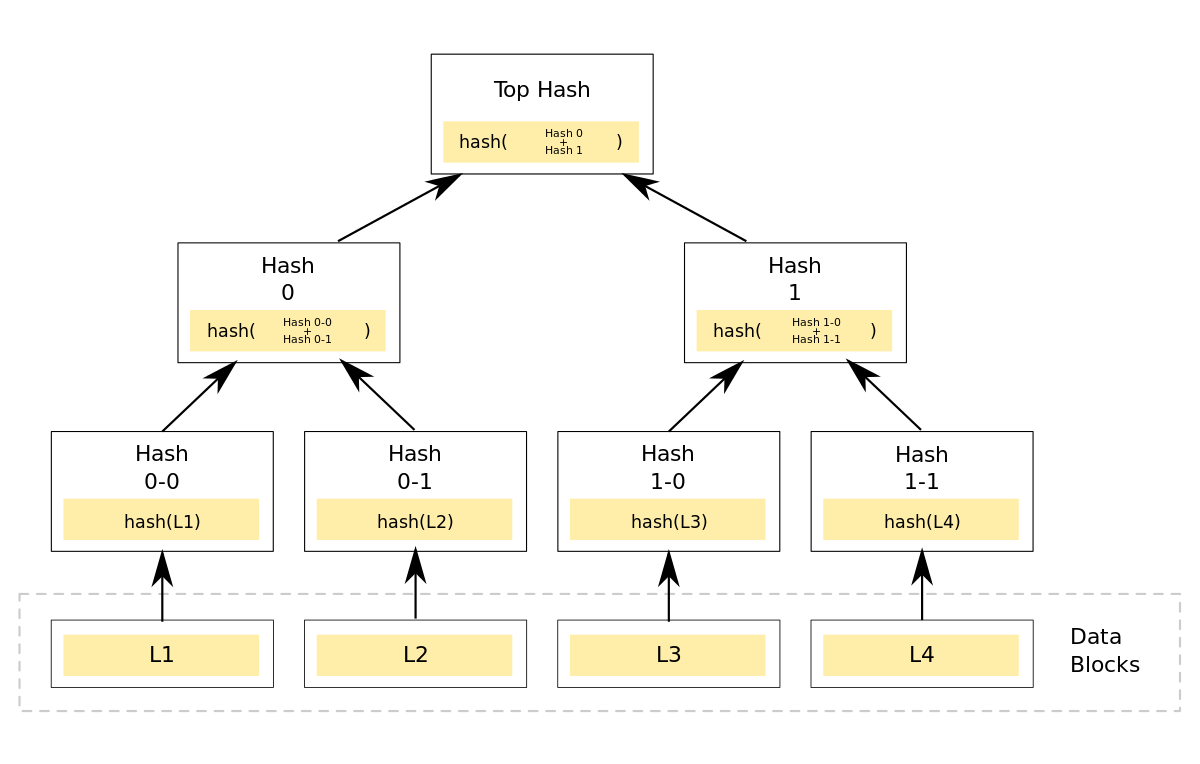
\includegraphics[width=0.9\textwidth]{Hash_Tree}
 	\caption{Một ví dụ của cây hash nhị phân.}
 \end{figure}

\subsection{Block}

Mỗi giao dịch trong tập giao dịch (tạo nên blockchain) được nạp vào một chương trình, tạo ra một mã được mã hóa được gọi là mã băm (hash value).\\
Các mã băm được kết lại hợp thành một cây Merkle.\\
Mã băm cuối cùng của tất cả quá trình băm này được đưa vào header của block, cùng với mã băm của header block trước nó và một tem thời gian.\\
Header này sau trở thành một phần của một bài đố mật mã học có lời giải là một con số gọi là "nounce".\\
Một khi lời giải đã được tìm ra thì block mới này sẽ được thêm vào blockchain


%\subsection{Block time}
%Block time là thời gian trung bình để tạo một block mới trong blockchain. 


\end{document}
